\documentclass[../BimodalReference.tex]{subfiles}
\begin{document}

\section{Introduction}

\textbf{TM} is a bimodal logic combining S5 a historical necessity operator ($\nec$) with linear temporal operators for past ($\allpast$) and future ($\allfuture$).
The logic provides a framework for reasoning about necessary truths across time to train AI systems to reason about past and future contingency.

The semantics is based on \emph{task frames}, which extend Kripke frames with temporal structure.
A task frame consists of world states connected by a \emph{task relation} indexed by temporal durations.
World histories are temporal slices through a task frame, representing the unfolding of a world over time.

\begin{center}
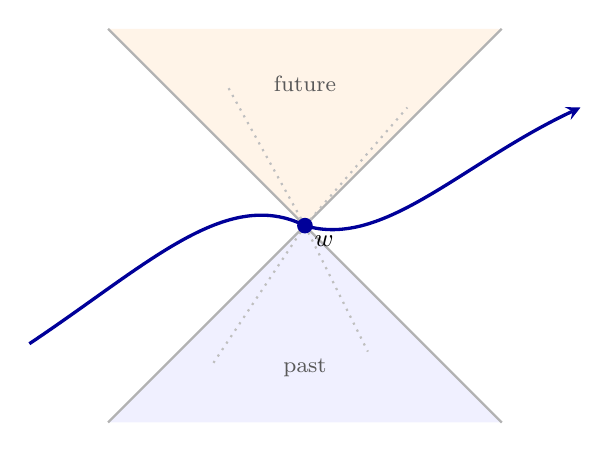
\begin{tikzpicture}[
  worldline/.style={very thick, blue!60!black},
  lightcone fill/.style={opacity=0.15},
  lightcone edge/.style={gray!60, thick},
  counterfactual/.style={dotted, thick, gray!50},
  point/.style={circle, fill=blue!60!black, inner sep=2pt}
]
  % Define the marked point P
  \coordinate (P) at (0,0);

  % Draw past light cone (filled region)
  \fill[blue!40, lightcone fill] (P) -- (-2.5,-2.5) -- (2.5,-2.5) -- cycle;

  % Draw future light cone (filled region)
  \fill[orange!60, lightcone fill] (P) -- (-2.5,2.5) -- (2.5,2.5) -- cycle;

  % Draw light cone boundary edges
  \draw[lightcone edge] (P) -- (-2.5,2.5);
  \draw[lightcone edge] (P) -- (2.5,2.5);
  \draw[lightcone edge] (P) -- (-2.5,-2.5);
  \draw[lightcone edge] (P) -- (2.5,-2.5);

  % Draw counterfactual past paths (dotted, within past cone)
  \draw[counterfactual] (P) -- (-1.2,-1.8);
  \draw[counterfactual] (P) -- (0.8,-1.6);

  % Draw alternative future paths (dotted, within future cone)
  \draw[counterfactual] (P) -- (-1.0,1.8);
  \draw[counterfactual] (P) -- (1.3,1.5);

  % Draw the S-shaped main worldline (actual history)
  \draw[worldline, ->, >=stealth] (-3.5,-1.5)
    .. controls (-2,-0.5) and (-1,0.5) .. (P)
    .. controls (1,-0.3) and (2,0.8) .. (3.5,1.5);

  % Draw the marked point P on top
  \node[point] at (P) {};
  \node[below right, font=\small] at (P) {$w$};

  % Labels for the cones
  \node[font=\footnotesize, gray!70!black] at (0,1.8) {future};
  \node[font=\footnotesize, gray!70!black] at (0,-1.8) {past};

\end{tikzpicture}
\end{center}

\noindent
The diagram above illustrates the conceptual structure underlying TM logic.
The solid curve represents a single world history---a temporal sequence of states.
From any point $w$ along a history, the past and future light cones contain all states that are modally accessible.
The necessity operator $\nec$ quantifies over all histories passing through $w$, while the temporal operators $\allpast$ and $\allfuture$ quantify along the single actual history.
The dotted lines represent counterfactual paths: alternative pasts that could have led to $w$, and alternative futures that could unfold from $w$.

\subsection*{Project Structure}

The Lean 4 implementation is in the \texttt{Bimodal/} directory:
\begin{itemize}
  \item \texttt{Syntax/} -- Defines the formula language with 6 primitive constructors and derived operators.
  \textbf{Complete.}
  \item \texttt{ProofSystem/} -- Axioms (14 schemata) and inference rules (7 rules) forming a Hilbert-style proof system.
  \textbf{Complete.}
  \item \texttt{Semantics/} -- Task frames model possible worlds; world histories model time; truth conditions define meaning.
  \textbf{Complete.}
  \item \texttt{Metalogic/} -- Soundness theorem (proven: all axioms valid, rules preserve validity), deduction theorem (proven: enables assumption introduction), and completeness infrastructure (Lindenbaum lemma, canonical model axiomatized).
  \textbf{Soundness and deduction complete; completeness pending.}
  \item \texttt{Theorems/} -- Perpetuity principles and modal theorems derived from the axiom system.
  \textbf{Partial.}
\end{itemize}

\end{document}
